\newpage
\subsection*{Question 3}

\begin{enumerate}[label={(\alph*)}]
    \item Here is the $B^+$-tree index :
    
        \begin{center}
            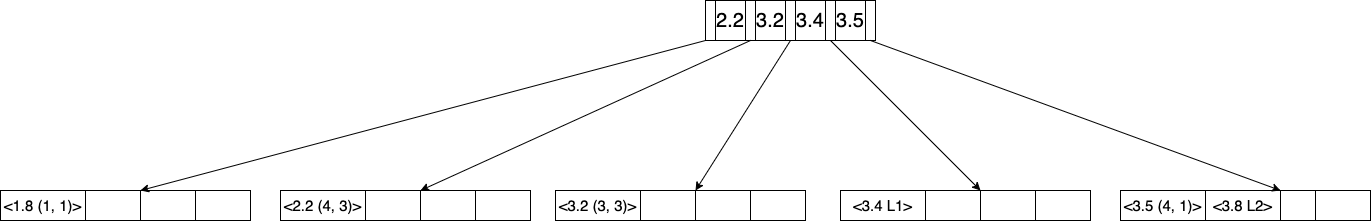
\includegraphics[width=1\textwidth]{img/img3.png}
        \end{center}
    
    \noindent The position of the tuples in the file (page \#, slot \#) are used to identify the different tuples. Note that for practical reasons, when a certain key (GPA) corresponds to a number of distinct entries that is too large, the list is replaced with a variable. List variables definitions are bellow: \\
    L1 = [(1, 3), (1, 4), (2, 1), (2, 2), (2, 3), (2, 4), (3, 1)]\\
    L2 = [(1, 2), (3, 2), (3, 4), (4, 2)]
    
    \item 
            \begin{enumerate}[label={\arabic*.}]
                \item If the tuples in $f$ are sorted, they will appear in the following order:\\
                    <1.8 (1, 1)> \\
                    <2.2, (1, 2)> \\
                    <3.2, (1, 3)> \\
                    <3.4 (1, 4), (2, 1), (2, 2), (2, 3), (2, 4), (3, 1), (3, 2)> \\
                    <3.5 (3, 3)> \\
                    <3.8, (3, 4), (4, 1), (4, 2), (4, 3)> \\
                    \noindent Hence, with the use of a $B^+$-tree index on GPA, the system would need to access 3 pages (pages 1, 2, and 3) before returning all values of tuples with a GPA between 3.0 and 3.5 inclusive.
                \item If the tuples in $f$ are not sorted, they will appear in the following order:\\
                        <1.8 (1, 1)> \\
                        <2.2, (4, 3)> \\
                        <3.2, (3, 3)> \\
                        <3.4 (1, 3), (1, 4), (2, 1), (2, 2), (2, 3), (2, 4), (3, 1)> \\
                        <3.5 (4, 1)> \\
                        <3.8, (1, 2), (3, 2), (3, 4), (4, 2)> \\
                    \noindent Hence, the system would need to access all 4 pages before returning all values of tuples with a GPA between 3.0 and 3.5 inclusive.
                \item We realize that the number of pages accessed is 33\% higher when tuples are unsorted in comparison to when they are sorted. This percentage quickly increases as the distribution of GPA widen and the number of tuples and tuples per page increases.
            \end{enumerate}
\end{enumerate}